An alteration of k-nearest neighbors density is where the density of each observation is relative to the average density of the nearby observations (ARD) as seen in eq.\eqref{eq:ARD}
\begin{equation}\label{eq:ARD}
    \text{ard}_\mathbf{X} (\mathbf{x}_i, K) = \frac{\text{density}_{\mathbf{X}_{\setminus i}} (\mathbf{x}_i, K) }{\frac{1}{K} \sum_{\mathbf{x}_j \in N_{\mathbf{X}_{\setminus i}} (\mathbf{x}_i, K)} \text{density}_{\mathbf{X}_{\setminus j}} (\mathbf{x}_j, K)}
\end{equation}

Using eq. \eqref{eq:ARD} we get the density scores and density distribution as seen in figure \ref{fig:ARD_DensityScore} and \ref{fig:ARD_DensityDistribution}, with the interval $[41.7, 268]$.

\begin{multicols}{2}
\begin{figure}[H]
    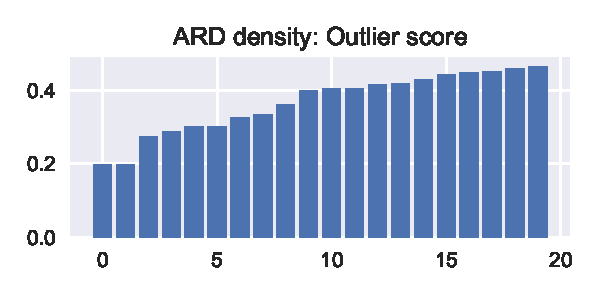
\includegraphics[width=\linewidth]{fig/ARD_densitybarplot_lowest20.pdf}
    \caption{20 lowest density scores using eq. \eqref{eq:ARD}.}
    \label{fig:ARD_DensityScore}
\end{figure}

\begin{figure}[H]
    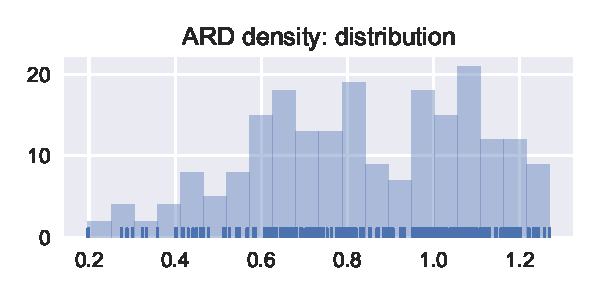
\includegraphics[width=\linewidth]{fig/ARD_densitydistribution.pdf}
    \caption{Density score distribution for the entire data set.}
    \label{fig:ARD_DensityDistribution}
\end{figure}
\end{multicols}

The interval of the density scores is much similar to the KNN method, but here the low density areas are a minority, and we see that the middle and higher dense areas are majorities. 